\chapter{System Model}\label{ch:system_model}

% ------------------------------------------------------------------------------
\section{System Model}\label{sec:system_model}
The system that will be considered throughout this work aims to represent the
downlink of a canonical cellular network, comprising several identical cells,
layed out over a regular hexagonal grid.

When studying a cellular network, the cells located at the edge of the network
will not experience the same conditions as the cells in the center of the
network. A typical way to deal with this situation is to consider a scenario
that wraps around (\reff{fig:torus_scenario}) so that cells on one side of the
scenario affect cells on the opposite side. Another option is to consider a
scenario with more cells than necessary, and then analyze the behavior of the
cells located within the center of the network (\reff{fig:interfering_scenario})
, so that the exterior cells account for the interference, equaling the
conditions of all the cells in the network.

\begin{figure}[t]
   \centering
   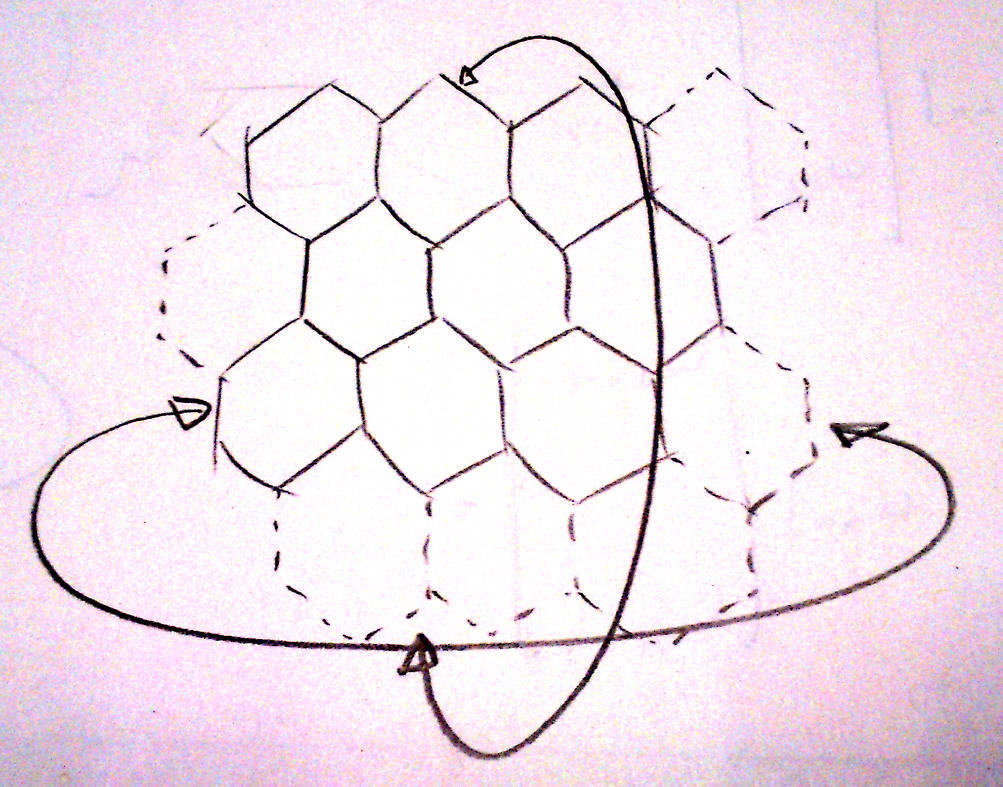
\includegraphics[width=0.5\textwidth]{./03.system_model/img/torus_scenario}
   \caption{Wrap around scenario. Cells on one side of the scenario influence
            the cells on the other side as if they were next to each other.}
   \label{fig:torus_scenario}
\end{figure}

\begin{figure}[t]
   \centering
   \includegraphics[width=0.5\textwidth]{./03.system_model/img/interfering_scenario}
   \caption{Oversized scenario. The behavior of the network is analyzed in the
            central cells of the network, and the exterior cells compensate the 
            network edge effects.}
   \label{fig:interfering_scenario}
\end{figure}

Each cell in the system under study will be served with a single \gls{bs} that
is equipped with $t$ transmit antennas. Each of the users considered in the
system has $r$ receive antennas.

A system with $M$ \gls{bs} and $N$ users can then be modelled as

\begin{equation} \label{eq:generic_system_model}
    \yy = \HH \xx + \nn
\end{equation}

$\yy$ represents the signal received at all the users and is defined as

\begin{equation} \label{eq:generic_rx_signal}
    \yy = \begin{bmatrix}
            \yy_1\\
            \vdots\\
            \yy_N
        \end{bmatrix} \in \C^{Nr \times 1}
\end{equation}

\noindent
where $\yy_i \in \C^{r \times 1}$ is the signal received at the $i$-th user.

$\HH$ is the channel matrix from all the \gls{bs} to all the users, with the
following structure

\begin{equation} \label{eq:generic_ch_mat}
    \HH = \begin{bmatrix}
            \HH_{11} & \cdots & \HH_{1M}\\
            \vdots   & \ddots & \vdots\\
            \HH_{N1}  & \cdots & \HH_{NM}
    \end{bmatrix} \in \C^{Nr \times Mt}
\end{equation}

\noindent
where $\HH_{ij} \in \C^{r \times t}$ represents the channel matrix from the
$j$-th \gls{bs} to the $i$-th user. It will include the path loss due to
propagation, small scale fading, shadowing, and any other characteristic of
the radio channel that needs to be taken into consideration.

$\xx$ is the signal transmitted from all the \gls{bs}, and it is composed of

\begin{equation} \label{eq:generic_tx_signal}
    \xx = \begin{bmatrix}
        \xx_1 \\
        \vdots \\
        \xx_M
    \end{bmatrix} \in \C^{Mt \times 1}
\end{equation}

\noindent
where $\xx_j \in \C^{t \times 1}$ is the signal transmitted by the $j$-th
\gls{bs}. Additionally, the power transmitted by the $j$-th \gls{bs} can be
calculated from the transmitted signal as

\begin{equation} \label{eq:bs_tx_power}
P_{j,\tx} = \Tr \left(\xx_j \xx_j^H\right) = \xx_j^H \xx_j
\end{equation}

\noindent
and each \gls{bs} will have an independent power constraint

\begin{equation} \label{eq:pbpc}
    P_{j,\tx} \leq P_{j, \max}
\end{equation}

Finally $\nn$ represents the \gls{awgn} at all the receivers

\begin{equation} \label{eq:generic_noise}
    \nn = \begin{bmatrix}
        \nn_1 \\
        \vdots \\
        \nn_N
    \end{bmatrix} \in \C^{Nr \times 1}
\end{equation}

\noindent
with $\nn_i \in \C^{r \times 1}$ accounts for the Gaussian noise at the $i$-th
receiver. Throughout this work $\nn_i$ is considered to be formed by \emph{iid}
entries, drawn from a zero mean, $\sigma_i^2$ variance Gaussian distribution,
$\nn_i \sim \mathcal{N}\left(\zero, \sigma_i^2 \eye\right)$. The noise variance
will be assumed the same for all the receivers.

In a general scenario, there may be cooperation among the \gls{bs} in the system
so that the information intended for a particular user will be transmitted by
several or all the \gls{bs}. Or, equivalently, each \gls{bs} transmits a
combination of the information of several users

\begin{equation} \label{eq:generic_tx_precod}
    \xx_j = \Wtx_{j1} \ss_1 + \cdots + \Wtx_{jN} \ss_N
\end{equation}

\noindent
where $\ss_i \in \C^{\ell \times 1}$ is the vector of information symbols to be
transmitted to user $i$, with $\ell$ being the number of simultaneous symbols or
streams to be transmitted to that user. $\Wtx_{ji} \in \C^{t \times \ell}$ is
the precoding matrix used at the $j$-th transmitter for the data of the
$i$-th user.

It will be assumed that the information symbols are independent and drawn from a
Gaussian distribution such that $\ss_i \sim \mathcal{N}\left(\zero, \RR_{\ss_i}
\right)$, where $\RR_{\ss_i} = \diag\left\{p_{i1}, \ldots, p_{i\ell}\right\} \in
\R^{\ell \times \ell}$ contains the power allocated to each of the symbols in
$\ss_i$. The transmitted power can be expressed as

\begin{equation} \label{eq:bs_precod_power}
    P_{j, \tx} = \sum\limits_{i=1}^{N} \Tr \left( \Wtx_{ji} \RR_{\ss_i}
    \WtxH_{ji} \right)
\end{equation}

The choice of the precoding matrices and of the receiving filter will determine
the transmission strategy used. This Thesis will focus mainly on \gls{bd}
\cite{spencer04} which is described in \refs{sec:bd}.

On the receiver side, no cooperation among the users will be considered, so each
user may perform, independently, additional processing of the received signal by
applying a linear filter or equalizer

\begin{equation} \label{eq:generic_rx_eq}
    \hat{\ss}_i = \Wrx_i \yy_i
\end{equation}

\noindent
where $\Wrx_i \in \C^{r \times \ell}$ is the equalizer used at the $i$-th
receiver.

Combining \eqref{eq:generic_system_model}--\eqref{eq:generic_tx_precod} it is
possible to rewrite \eqref{eq:generic_system_model} as

\begin{equation} \label{eq:system_model}
    \yy = \HH \Wtx \ss + \nn
\end{equation}

\noindent
where

\begin{equation} \label{data_symbols}
    \ss = \begin{bmatrix}
        \ss_1 \\
        \vdots \\
        \ss_N
    \end{bmatrix} \in \C^{N\ell \times 1}
\end{equation}

\noindent
and the global precoding matrix is

\begin{equation} \label{eq:precoding_matrix}
    \Wtx = \begin{bmatrix}
        \Wtx_{11} & \cdots & \Wtx_{1N} \\
        \vdots    & \ddots & \vdots \\
        \Wtx_{M1} & \cdots & \Wtx_{MN} \\
    \end{bmatrix} \in \C^{Mt \times N\ell}
\end{equation}

\noindent
and it can be partitioned as

\begin{equation} \label{eq:precod_partition}
    \Wtx = \left[ \Wtx_1, \ldots, \Wtx_N \right]
\end{equation}

\noindent
with

\begin{equation} \label{eq_precod_user}
    \Wtx_i = \begin{bmatrix}
        \Wtx_{11} \\
        \vdots \\
        \Wtx_{M1}
    \end{bmatrix} \in \C^{Mt \times \ell}
\end{equation}

The channel matrix can then be partitioned as

\begin{equation} \label{eq:ch_mat_partition}
    \HH = \begin{bmatrix}
        \HH_1 \\
        \vdots \\
        \HH_N
    \end{bmatrix}
\end{equation}

\noindent
where $\HH_i \in \C^{r \times Mt}$ is the channel matrix from all the \gls{bs}
to the $i$-th user.

As it has already been mentioned, receiver cooperation is not going to be
considered, so looking at a particular user, \emph{e.g.} the $i$-th user, the
signal that is received will be

\begin{equation} \label{eq:rx_signal_user}
    \yy_i = \HH_i \Wtx \ss + \nn_i
\end{equation}

\noindent
which can be rewritten as

\begin{equation} \label{eq:rx_signal_user_interf}
    \yy_i = \HH_i \Wtx_i \ss_i +
    \underbrace{\sum\limits_{\substack{j = 1\\j \neq i}}^{N} \HH_i
        \Wtx_j \ss_j}_{\text{Interference}} + \nn_i
\end{equation}

\noindent
so that it can be readily seen how other users' data appear as an interference
term that degrades the received signal.

Defining the term of interference plus noise as

\begin{equation} \label{eq:interf_plus_noise}
    \zz_i = \sum\limits_{\substack{j = 1\\j \neq i}}^{N} \HH_i \Wtx_j
    \ss_j + \nn_i
\end{equation}

and using \eqref{eq:rx_signal_user_interf}, the ergodic (mean) rate for the
$i$-th user is given by \cite{cover_thomas}, \cite{holter01}

\begin{equation} \label{eq:generic_ergodic_capacity}
    R_i = \mathbb{E}\left\{
        \log_2\left| \eye + \HH_i\Wtx_i\RR_{\ss_i}\WtxH_i\HH_i^H \RR_{\zz_i}^{-1}
    \right|
    \right\}
\end{equation}

\noindent
where $\RR_{\zz_i} \in \C^{r \times r}$ is the covariance matrix of the noise plus
the interference term in \eqref{eq:rx_signal_user_interf}

\begin{equation} \label{eq:r_in}
    \RR_{\zz_i} = \zz_i \zz_i^H = 
    \left(\sum\limits_{\substack{j=1\\j\neq i}}^{N} \HH_i\Wtx_j+\nn_i
    \right)
    \left(\sum\limits_{\substack{j=1\\j\neq i}}^{N} \HH_i\Wtx_j+\nn_i
    \right)^H
\end{equation}

In the rest of the work, there are a set of assumptions that will be made,
mainly to guarantee the feasibility of some of the results obtained:

\begin{itemize}
    \item The number of users will be the same as the number of \gls{bs},
        \emph{i.e.} $N = M$.
    \item The total number of antennas transmitting will be greater or equal
        than the total number of antennas at the receiver side, this is $Mt
		\geq Nr$.
    \item The number of streams transmitted to each user must be $\ell \leq r$.
    \item There is no correlation, neither at the transmitters nor at the
        receivers, so that $\HH$ is full rank or, equivalently, $\rank\left(
        \HH\right) = \min\left(Nr,Mt\right)$. As $Mt \geq Nr$, then $\rank\left(
        \HH\right) = Nr$.
\end{itemize}

% ------------------------------------------------------------------------------
\section{Block Diagonalization}\label{sec:bd}

One possibility to cancel the inter-user interference is to diagonalize the
channel matrix. Perfect diagonalization is only possible if $Mt \geq Nr$
\cite{caire03}, and it is achieved using the following precoding matrix

\begin{equation} \label{eq:zf_precod}
    \Wtx = \HH^\dagger
\end{equation}

This solution is optimum only when every user has only one antenna. In the case
under study, with multiantenna receivers, complete diagonalization of the
channel matrix is suboptimal since each user is able to coordinate the
processing of its received signal.

In \cite{spencer04} is stated that the optimum solution under the constraint
that all inter-user interference be zero is obtained with $\HH \Wtx$ being
block diagonal. In \cite{spencer04}, \gls{bd} is proposed as an algorithm to
obtain a precoding matrix that is able to block diagonalize the channel matrix.
This algorithm is described next.

In order to meet the condition of zero inter-user interference, it is necessary
to cancel the interference term in \eqref{eq:rx_signal_user_interf}, and this
is equivalent to meet the following

\begin{equation} \label{eq:cancel_interf}
    \HH_i \Wtx_j = \zero \text{\quad } \forall j \neq i
\end{equation}

Let $\Htilde_i$ be the channel matrix $\HH$ without $\HH_i$, \emph{i.e.}

\begin{equation} \label{eq:h_tilde}
    \Htilde_i = \begin{bmatrix}
        \HH_1 \\
        \vdots \\
        \HH_{i - 1} \\
        \HH_{i + 1} \\
        \vdots \\
        \HH_N
    \end{bmatrix} \in \C^{(N - 1)r \times Mt}
\end{equation}

Then the condition \eqref{eq:cancel_interf} can be obtained making $\Wtx_i$ lie
in the null space or kernel of $\Htilde_i$. This is possible only if the
dimension of the null space is greater than zero, \emph{i.e.} $\rank\left(\ker
\left(\Htilde_i\right)\right) > 0$.

Now, with the dimensions of $\Htilde$, the rank of its null space is

\begin{equation} \label{eq:rank_kern_htilde}
   \rank\left(\ker\left(\Htilde_i\right)\right) = Mt - \rank\left(\Htilde_i
   \right)
\end{equation}

But it is assumed that $\HH$ is full rank, ergo $\rank\left(\Htilde_i\right) =
(N - 1)r = \Ltilde_i$, and then

\begin{equation} \label{eq:rank_kern_htilde_ok}
    \rank\left(\ker\left(\Htilde_i\right)\right) = Mt - \Ltilde_i > 0
\end{equation}

\noindent
so it is guaranteed that a precoding matrix $\Wtx_i$ that lies in the null space
of $\Htilde_i$ exists.

The simplest way to obtain such $\Wtx_i$ involves using the \gls{svd} of the
matrix $\Htilde_i$.

Let $\Htilde_i$ be decomposed as

\begin{equation} \label{eq:htilde_svd}
    \Htilde_i = \Utilde_i \bLambdatilde_i \left[ \Vtilde_i^{(1)}, \Vtilde_i^{(0)}
    \right]^H
\end{equation}

\noindent
where $\Vtilde_i^{(0)} \in \C^{Mt \times (Mt - \Ltilde_i)}$ contains the last
$Mt - \Ltilde_i$ right singular vectors of $\Htilde_i$, corresponding to the
singular values equal to zero. $\Vtilde_i^{(0)}$ forms an orthonormal basis of
the null space of $\Htilde_i$, and thus its columns can be used to cancel the
inter-user interference

\begin{equation} \label{eq:v0_zero_interf}
    \Htilde_i \Vtilde_i^{(0)} = \zero
\end{equation}

Using these matrices as precoding the result is

\begin{equation} \label{eq:block_diag}
    \Hhat = \HH \begin{bmatrix}
        \Vtilde_1^{(0)}, \ldots, \Vtilde_N^{(0)}
    \end{bmatrix} = \begin{bmatrix}
        \HH_1 \Vtilde_1^{(0)} &        & \zero \\
                              & \ddots & \\
        \zero                 &        & \HH_N \Vtilde_N^{(0)}
    \end{bmatrix}
\end{equation}

\noindent
that, as it can be seen, has a block diagonal structure, which gives the name to
the algorithm proposed in \cite{spencer04}.

The next problem that \gls{bd} solves is the maximization of the sum rate of the
system, given the block diagonal structure in \eqref{eq:block_diag}. The
precoding matrix $\Wtx_i$ will be considered to be

\begin{equation} \label{eq:wtx_nosvd}
    \Wtx_i = \Vtilde_i^{(0)} \WW_i^{\prime}
\end{equation}

\noindent
where $\WW_i^{\prime} \in \C^{(Mt - \Ltilde_i) \times \ell}$ will take care of
the rate maximization.

Introducing \eqref{eq:wtx_nosvd} into \eqref{eq:generic_ergodic_capacity} the
ergodic capacity simplifies to

\begin{equation} \label{eq:bd_ergodic_capacity_nosvd}
    R_i^{\text{no interf}} = \mathbb{E}\left\{
        \log_2\left| \eye + \frac{1}{\sigma_i^2}\Hhat_i\WW_i^{\prime}
        \RR_{\ss_i} \WW_i^{\prime,H}\Hhat_i^H
    \right|
    \right\}
\end{equation}

\noindent
where $\Hhat_i = \HH_i\Vtilde_i^{(0)} \in \C^{r \times (Mt - \Ltilde_i)}$.

In order to maximize the rate, consider the \gls{svd}

\begin{equation} \label{eq:svd_max_rate}
    \Hhat_i = \Uhat_i \begin{bmatrix}
        \bLambdahat_i & \zero \\
        \zero        & \zero
    \end{bmatrix} \left[ \Vhat_i^{(1)}, \Vhat_i^{(0)} \right]^H
\end{equation}

\noindent
where $\bLambdahat_i = \diag\left\{\lambdahatsqrt_{i1}, \ldots,
\lambdahatsqrt_{ir} \right\} \in \C^{r \times r}$ contains the non zero singular
values of $\Hhat_i$ , which has $\rank\left(\Hhat_i\right) = r$. And
$\Vhat_i^{(1)} \in \C^{(Mt - \Ltilde_i) \times r}$ contains the first $r$ right
singular vectors of $\Hhat_i$ , and it will be used as $\WW_i^{\prime}$,
yielding the following precoding matrix

\begin{equation} \label{eq:bd_precod}
    \Wtx_i = \Vtilde_i^{(0)} \Vhat_i^{(1)}
\end{equation}

The \gls{bd} also provides the receiver filter to be used at each user which
will be

\begin{equation} \label{eq:bd_eq}
    \Wrx_i = \Uhat_i^H
\end{equation}

Using all of the above, the rate that the $i$-th user can obtain is given by the
expression

\begin{equation} \label{eq:bd_ergodic_capacity}
    R_i^{\text{BD}} = \mathbb{E}\left\{
        \sum\limits_{k = 1}^{\ell} \log_2 \left(1 + \frac{\lambdahat_{ik}
        p_{ik}}{\sigma_i^2} \right)
    \right\}
\end{equation}

\noindent
where the only parameters left to be computed are the power allocated to each of
the $\ell$ streams of each user, and different options to do it will be
discussed in \refs{sec:power_allocation}.

% ------------------------------------------------------------------------------
\section{Power Allocation}\label{sec:power_allocation}

In \refs{sec:bd}, the \gls{bd} algorithm has been described to get the precoding
matrix to be used at the transmitter and the equalization filter to be used at
the receiver side. After \gls{bd} has been used, the power should be allocated
to each of the data streams of each user, this is, the $p_{ij}$ in
\eqref{eq:bd_ergodic_capacity} should be calculated in order to achieve a given
performance, and subject to particular constraints.

The need for a power allocation algorithm comes from the restriction on the
maximum power available for transmission, which may be due to physical
limitations, or regulatory issues.

There are several different power constraints:

\begin{itemize}
    \item \gls{papc}: The maximum power is constrained for each antenna at the
        transmitter. This option is specially well suited for distributed
        antenna systems \cite{choi07}, \cite{lee12}.
    \item \gls{pbpc}: In this case the maximum power is limited per base station
        instead of per antenna. This option is more appropriate for scenarios
        where all the transmitting antennas are collocated and may share a power
        budget, so that the transmission power can be arbitrarily allocated to
        each of the transmitter antennas.
\end{itemize}

A \gls{tpc} can also be considered, which assumes that the maximum power is
shared among all the transmitters in the system. Although this system is more
easily analyzed, it is very unrealistic so it will not be considered in this
work, except in \refss{ssec:scaled_wf} where a \gls{tpc} is used to obtain an
intermediate result.

For the sake of simplicity, \gls{pbpc} will be used for the different analyses. In any case, \gls{papc} can be seen as a particularization of \gls{pbpc} as the
derivations shown in this section can be applied to a \gls{papc} system
considering instead of each \gls{bs} to have $t$ transmit antennas, $t$ single
antenna \gls{bs}.

The problem that needs to be solved is, in general, the maximization of some
function of the rate of each of the users subject to a \gls{pbpc}

\begin{equation} \label{eq:generic_optim_problem}
\begin{aligned}
	&\maxi\limits_{\left\{\RR_{\ss_i}\right\}} &&\quad f\left(R_i^{\text{BD}}
    \left(\RR_{\ss_1},\right), \ldots, R_N^{\text{BD}}\left(\RR_{\ss_N}\right)
    \right) \\
	&\st &&\quad P_{j, \tx} \leq P_{j, \max},\quad j = 1, \ldots, M
\end{aligned}
\end{equation}

One common metric used for the maximization is the weighted sum-rate of the
system, so that the function $f\left(\cdot\right)$ is equal to

\begin{equation} \label{eq:weighted_sum_rate}
    f\left(R_i^{\text{BD}}, \ldots, R_N^{\text{BD}}\right) =
    \sum\limits_{i = 1}^{N}\alpha_i R_i^{\text{BD}}
\end{equation}

\noindent
where $\alpha_i \in \left[0, 1\right]$ can be seen as different priorities for
different users, and they are assumed to be

\begin{equation} \label{eq:priorities}
    \sum\limits_{i = 1}^{N}\alpha_i = 1
\end{equation}

\noindent
and in the particular case where all the $\alpha_i = 1/N$, then the function
$f\left(\cdot\right)$ represents the sum-rate of the system.

Calling

\begin{equation} \label{eq:precoding_bs}
	\WtxBar_j = \left[\Wtx_{j1}, \ldots, \Wtx_{jN}\right] \in \C^{t \times
	N\ell}
\end{equation}

\noindent
the precoding matrix of the $j$-th \gls{bs}, and

\begin{equation} \label{eq:powers_all_users}
	\RR_{\ss} = \blkdiag \left(\RR_{\ss_1}, \ldots, \RR_{\ss_N}\right) \in
	\C^{N\ell \times N\ell}
\end{equation}

\noindent
the matrix containing the power assigned to all the streams of all the users,
the power constraint in \eqref{eq:generic_optim_problem} can then be
reformulated as

\begin{equation} \label{eq:pbpc_constraint}
	\Tr \left( \WtxBar_j\RR_{\ss}\WtxHbar_j \right) \leq P_{j,\max}
\end{equation}

Now the term inside the trace operator can be written explicitly as a function
of $p_{ik}$ in order to make it easier to analyze. First define

\begin{equation} \label{eq:precoding_bs_columns}
	\WtxBar_j = \left[ \wbar_{j,11}, \ldots, \wbar_{j, 1\ell}, \ldots,
	\wbar_{j,N\ell} \right]
\end{equation}

\noindent
where $\wbar_{j, ik} \in \C^{t \times 1}$ is the $ik$-th column of $\WtxBar_j$,
\emph{i.e.} the precoding that is used at the $j$-th \gls{bs} for the $k$-th
stream of the $i$-th user.
And then:

\begin{equation}
\begin{aligned}
	\WtxBar_j\RR_{\ss}\WtxHbar_j = &\left[\wbar_{j,11}, \ldots, \wbar_{j, N\ell}
	\right]
	\begin{bmatrix}
		p_{11} &        & 0\\
               & \ddots &  \\
		0      &        & p_{N\ell}

	\end{bmatrix}
	\begin{bmatrix}
		\wbar_{j,11}^H\\
		\vdots\\
		\wbar_{j,N\ell}^H
	\end{bmatrix} = \\
	= & p_{11}\wbar_{j,11}\wbar_{j,11}^H + \cdots + p_{N\ell}\wbar_{j,N\ell}
	\wbar_{j,N\ell}^H \\
	= & \sum\limits_{i = 1}^N\sum\limits_{k = 1}^\ell p_{ik}
	\wbar_{j,ik}\wbar_{j,ik}^H
\end{aligned}
\end{equation}

\noindent
and the trace is

\begin{equation} \label{eq:trace_terms_p_i}
	\Tr\left(\WtxBar_j \RR_{\ss} \WtxHbar_j\right) = \sum\limits_{i = 1}^N
	\sum\limits_{k = 1}^\ell p_{ik} \left\| \wbar_{j, ik} \right\|_2^2
\end{equation}

\noindent
where

\begin{equation} \label{eq:norm2}
    \left\|\wbar_{j,ik}\right\|_2^2 = \Tr\left( \wbar_{j,ik} \wbar_{j,ik}^H
    \right) = \wbar_{j,ik}^H \wbar_{j,ik}.
\end{equation}

The sum-rate maximization problem can then be formulated in \emph{standard form}
\cite{boyd_convex} as

\begin{equation} \label{eq:sum_rate_maxim}
\begin{aligned}
	&\mini\limits_{p_{ik}} &&-\sum\limits_{i = 1}^N
	\sum\limits_{k = 1}^\ell \log_2\left( 1 +
	\frac{\lambdahat_{ik} p_{ik}}{\sigma_i^2} \right)\\
	&\st &&\sum\limits_{i = 1}^N \sum\limits_{k = 1}^\ell p_{ik} \left\|
	\wbar_{j,ik} \right\|_2^2 - P_{j,\max} \leq 0, &&
    \begin{array}{l}
        j = 1, \ldots, M
    \end{array}\\
    & &&-p_{ik} \leq 0, &&
	\begin{array}{l}
	i = 1, \ldots, N\\
	k = 1, \ldots, \ell
	\end{array}
\end{aligned}
\end{equation}

In the next sections, different alternatives for obtaining these powers are
presented and described.

% ------------------------------------------------------------------------------
\subsection{Optimal Power Allocation}\label{ssec:optimal_power_allocation}

In \eqref{eq:sum_rate_maxim}, the function $\log_2(\cdot)$ is convex on $p_{ik}$
 and the sum of convex functions is also convex, so the objective function in
\eqref{eq:sum_rate_maxim} is convex. The constraints are affine and therefore
convex too. The optimization problem in \eqref{eq:sum_rate_maxim} is a convex
optimization problem that can be solved using a myriad of numerical technics
\cite{boyd_convex}. Nonetheless, it would be interesting to analyze a bit
further the problem in order to get some insight about it.

The problem in \eqref{eq:sum_rate_maxim} satisfies \emph{Slater's condition}
\cite{boyd_convex} since the objective function is convex and all the
inequality constraints are affine, hence \emph{strong duality} holds. This means
that the optimum value of the primal problem is equal to the optimum value of
the \emph{Lagrange dual problem}, so that this can be used to find out the
solution to the primal, original, problem.

Under these conditions, and considering that the objective function is
differentiable with respect to $p_{ik}$, \gls{kkt} conditions \cite{boyd_convex}
are necessary and sufficient for optimality of a solution, and they can be used
to analyze the optimization problem in search for an optimal solution. The
\gls{kkt} conditions for \eqref{eq:sum_rate_maxim} are

\begin{equation} \label{eq:kkt_conditions}
\begin{array}{rccl}
	\sum\limits_{i = 1}^N \sum\limits_{k = 1}^\ell p_{ik}^\ast \left\|
    \wbar_{j,ik} \right\|_2^2 - P_{j,\max} & \leq & 0, &
    \begin{array}{l}
        j = 1, \ldots, M
    \end{array}\\

    p_{ik}^\ast &\leq & 0, &
	\begin{array}{l}
	i = 1, \ldots, N\\
	k = 1, \ldots, \ell
	\end{array}\\

    \nu_j^\ast & \geq & 0, &
    \begin{array}{l}
        j = 1, \ldots, M
    \end{array}\\

    \mu_{ik}^\ast & \geq & 0, &
	\begin{array}{l}
	i = 1, \ldots, N\\
	k = 1, \ldots, \ell
	\end{array}\\

    \nu_j^\ast\left(\sum\limits_{i = 1}^N \sum\limits_{k = 1}^\ell p_{ik}
    \left\|\wbar_{j,ik} \right\|_2^2 - P_{j,\max} \right) & = & 0, &
    \begin{array}{l}
        j = 1, \ldots, M
    \end{array}\\

    -\mu_{ik}^\ast p_{ik}^\ast & = & 0, &
	\begin{array}{l}
	i = 1, \ldots, N\\
	k = 1, \ldots, \ell
	\end{array}\\

    \nablabf_{\pp} \mathcal{L}\left(\pp^\ast, \mathbf{\nu}^\ast,
        \mathbf{\mu}^\ast \right) & = & \zero

\end{array}
\end{equation}

\noindent
where the superscript $^\ast$ represents a feasible solution of the optimization
problem, $\nablabf_{\pp}$ is the gradient with respect to the powers $\pp = 
\left[p_{11}, \ldots, p_{N\ell}\right]^T$, $\mathbf{\nu} = \left[\nu_1, \ldots,
\nu_M\right]^T$ and $\mathbf{\mu} = \left[\mu_{11}, \ldots, \mu_{N\ell}
\right]^T$ are the Lagrange multipliers, and $\mathcal{L}$ represents the
\emph{Lagrangian} associated with the problem \eqref{eq:sum_rate_maxim}, and it
is defined as

\begin{equation} \label{eq:lagrangian}
\begin{aligned}
    \mathcal{L}\left(\pp, \mathbf{\nu}, \mathbf{\mu}\right) =
    & -\sum\limits_{i = 1}^N
        \sum\limits_{k = 1}^\ell \log_2\left( 1 +
        \frac{\lambdahat_{ik} p_{ik}}{\sigma_i^2} \right) + \\
    & \sum\limits_{j = 1}^M \nu_j\left(
        \sum\limits_{i = 1}^N \sum\limits_{k = 1}^\ell p_{ik} \left\|
        \wbar_{j,ik} \right\|_2^2 - P_{j,\max}\right) - \\
    & \sum\limits_{i = 1}^N \sum\limits_{k = 1}^\ell \mu_{ik} p_{ik}
\end{aligned}
\end{equation}

The gradient of a function $f(\xx)$ with respect to $\xx \in \C^{n \times 1}$ is
defined as

\begin{equation} \label{eq:gradient}
    \nablabf_{\xx}f(\xx) = \begin{bmatrix}
        \frac{\partial}{\partial x_1}f(\xx) \\
        \vdots \\
        \frac{\partial}{\partial x_n}f(\xx)
    \end{bmatrix}
\end{equation}

First the gradient of the objective function is calculated, by computing the
partial derivatives

\begin{equation} \label{eq:gradient_objective}
    \frac{\partial}{\partial p_{ik}} \left\{
        -\sum\limits_{i = 1}^N
        \sum\limits_{k = 1}^\ell \log_2\left( 1 +
        \frac{\lambdahat_{ik} p_{ik}}{\sigma_i^2} \right)
    \right\} = \frac{-\lambdahat_{ik}}{\ln\left(2\right)\left(\sigma_i^2 +
    \lambdahat_{ik} p_{ik}\right)}
\end{equation}

And the same for the inequality constraints

% The comment in the middle of the `aligned` environment is intended so that it
% does not fail compiling
\begin{equation} \label{eq:gradient_constraints}
\begin{aligned}
    &\frac{\partial}{\partial p_{ik}} \left\{
    \sum\limits_{i = 1}^N \sum\limits_{k = 1}^\ell p_{ik}
    \left\| \wbar_{j,ik} \right\|_2^2 - P_{j,\max}
    \right\} = \left\| \wbar_{j,ik} \right\|_2^2 \\
%
    &\frac{\partial}{\partial p_{ik}} \left\{ p_{ik} \right\} = 1
\end{aligned}
\end{equation}

So that the condition of the gradient of the Lagrangian vanishing, in
\eqref{eq:sum_rate_maxim} can be writen as

\begin{equation} \label{eq:gradient_vanishing}
    \frac{-\lambdahat_{ik}}{\ln\left(2\right)\left(\sigma_i^2 +
    \lambdahat_{ik} p_{ik}^\ast\right)} +
    \sum\limits_{j = 1}^M \nu_j^\ast \left\|\wbar_{j, ik}\right\|_2^2 -
    \mu_{ik}^\ast = 0,\quad
	\begin{array}{l}
	i = 1, \ldots, N\\
	k = 1, \ldots, \ell
	\end{array}\\
\end{equation}

It can be seen that $\mu_{ik}$ is a slack variable that takes into account the
non-negativeness of the powers $p_{ik}$, and it can be ommited to get the
equation

\begin{equation} \label{eq:gradient_inequality}
    \frac{-\lambdahat_{ik}}{\ln\left(2\right)\left(\sigma_i^2 +
    \lambdahat_{ik} p_{ik}^\ast\right)} +
    \sum\limits_{j = 1}^M \nu_j^\ast \left\|\wbar_{j, ik}\right\|_2^2
    \geq 0,\quad
	\begin{array}{l}
	i = 1, \ldots, N\\
	k = 1, \ldots, \ell
	\end{array}\\
\end{equation}

Calling

\begin{equation} \label{eq:term_columns_w}
    L_{ik} = \sum\limits_{j = 1}^M \nu_j^\ast \left\|\wbar_{j, ik}\right\|_2^2
\end{equation}

\noindent
\eqref{eq:gradient_inequality} can be solved for $p_{ik}^\ast$

\begin{equation} \label{eq:optimum_p}
    p_{ik}^\ast \leq \frac{1}{\ln\left(2\right)L_{ik}} - \frac{\sigma_i^2}
    {\lambdahat_{ik}}, \quad
	\begin{array}{l}
	i = 1, \ldots, N\\
	k = 1, \ldots, \ell
	\end{array}\\
\end{equation}

The result in \eqref{eq:optimum_p} resembles the classical \emph{water-filling}
solution, except that now the water level is not fixed, and it depends on the
precoders. The coupling existing among the power constraints of the different
\gls{bs} makes it impossible to find a closed-form solution for the values of
$p_{ik}$.

Nevertheless, this analysis motivates the development of suboptimal schemes that are described in the following sections.

% ------------------------------------------------------------------------------
\subsection{Modified Water-Filling}\label{ssec:modified_wf}

\cite{armada11b} proposes a simplification to the original problem, in order to
make it more tractable. The coupling of the power constraints in
\eqref{eq:sum_rate_maxim} makes it impossible to get a simple solution for the
optimal power allocation problem. \cite{armada11b} approaches the problem by
first considering an equivalent virtual \gls{bs} so that the problem is cast
with a single power constraint.

In order to do so, instead of having a power constraint for each of the \gls{bs}
consider a single power constraint given by the most restrictive \gls{bs} in the
original problem. Define

\begin{equation} \label{eq:equiv_bs}
    \OmegaEq = \max\limits_{j=1, \ldots,M} \left\|\wbar_{j,ik} \right\|_2^2
\end{equation}

\noindent
as the weights of the single virtual \gls{bs} corresponding to each of the
users' streams. The optimization problem becomes then

\begin{equation} \label{eq:optim_modif_wf}
\begin{aligned}
	&\mini\limits_{p_{ik}} &&-\sum\limits_{i = 1}^N
	\sum\limits_{k = 1}^\ell \log_2\left( 1 +
	\frac{\lambdahat_{ik} p_{ik}}{\sigma_i^2} \right)\\
	&\st &&\sum\limits_{i = 1}^N \sum\limits_{k = 1}^\ell p_{ik} \OmegaEq -
    P_{\text{BS},\max} \leq 0\\
    & &&-p_{ik} \leq 0, &&
	\begin{array}{l}
	i = 1, \ldots, N\\
	k = 1, \ldots, \ell
	\end{array}
\end{aligned}
\end{equation}

\noindent
where $P_{\text{BS}, \max}$ represents the most restrictive power constraint
among all of the \gls{bs}.

This problem meets the same conditions as the original problem so that a similar
analysis can be used. First formulate the Lagrangian of the new problem as

\begin{equation} \label{eq:modif_wf_lagrangian}
\begin{aligned}
    \mathcal{L}\left(\pp, \nu, \mathbf{\mu}\right) =
    & -\sum\limits_{i = 1}^N
        \sum\limits_{k = 1}^\ell \log_2\left( 1 +
        \frac{\lambdahat_{ik} p_{ik}}{\sigma_i^2} \right) + \\
    & \nu\left(
        \sum\limits_{i = 1}^N \sum\limits_{k = 1}^\ell p_{ik} \OmegaEq -
        P_{\text{BS},\max}\right) - \\
    & \sum\limits_{i = 1}^N \sum\limits_{k = 1}^\ell \mu_{ik} p_{ik}
\end{aligned}
\end{equation}

And its gradient is given by

\begin{equation} \label{eq:modif_wf_gradient}
    \nablabf_{\pp} \mathcal{L}\left(\pp^\ast, \nu^\ast, \mathbf{\mu}^{\ast}
    \right) = 
    \frac{-\lambdahat_{ik}}{\ln\left(2\right)\left(\sigma_i^2 +
    \lambdahat_{ik} p_{ik}^\ast\right)} +
    \nu^\ast \OmegaEq - \mu_{ik}^\ast = 0,\quad
	\begin{array}{l}
	i = 1, \ldots, N\\
	k = 1, \ldots, \ell
	\end{array}\\
\end{equation}

Using the \gls{kkt} condition that the gradient of the Lagrangian should vanish,
and considering $\mu_{ik}^\ast$ a slack variable, and solving for $p_{ik}^\ast$,
the following inequality is obtained

\begin{equation} \label{eq:modified_wf_gradient_ineq}
    p_{ik}^\ast \leq \frac{1}{\ln\left(2\right)\nu^\ast\OmegaEq} -
    \frac{\sigma_i^2}{\lambdahat_{ik}}, \quad 
	\begin{array}{l}
	i = 1, \ldots, N\\
	k = 1, \ldots, \ell
	\end{array}
\end{equation}

\noindent
which, together with the constraint of the powers being non-negative, can be
written as

\begin{equation} \label{eq:mwf}
    p_{ik}^\ast = \left[\frac{1}{\ln\left(2\right)\nu^\ast\OmegaEq} - 
    \frac{\sigma_i^2}{\lambdahat_{ik}}\right]^+, \quad 
	\begin{array}{l}
	i = 1, \ldots, N\\
	k = 1, \ldots, \ell
	\end{array}
\end{equation}

The solution of this simplified problem is given by the water-filling solution
with a variable water level and, in this case, an uncoupled solution for each of
the data streams for each user. This allows for the use of standard and
efficient methods to find the power allocation \cite{cioffi_notes}.

Clearly, the definition of the new problem makes it more restrictive than the
original, and its solution will be also a feasible solution for the original
problem, albeit not the optimal. The results in \cite{armada11b} show how under
some conditions, the solution achieved like this can be rather close to the
optimum one.

% ------------------------------------------------------------------------------
\subsection{Scaled Water-Filling}\label{ssec:scaled_wf}

In \cite{zhang09} the same power allocation problem as in
\eqref{eq:sum_rate_maxim} is dealt with by considering a \gls{tpc}, so that the
optimization problem becomes

\begin{equation} \label{eq:optim_scaled_wf}
\begin{aligned}
	&\mini\limits_{p_{ik}} &&-\sum\limits_{i = 1}^N
	\sum\limits_{k = 1}^\ell \log_2\left( 1 +
	\frac{\lambdahat_{ik} p_{ik}}{\sigma_i^2} \right)\\
    &\st && \Tr\left( \Wtx \RR_{\ss} \WtxH \right) - M P_{\max} \leq 0\\
    & &&-p_{ik} \leq 0, &&
	\begin{array}{l}
	i = 1, \ldots, N\\
	k = 1, \ldots, \ell
	\end{array}
\end{aligned}
\end{equation}

\noindent
where it has been assumed that $P_{j,\max} = P_{\max} \forall j$.

Under this \gls{tpc}, the solution is readily derived by water-filling
\cite{cioffi_notes}, but the resulting $\RR_{\ss}^{\text{TPC}}$ may violate
the individual power contraints of each \gls{bs}.

In order to meet each \gls{pbpc}, the matrix $\RR_{\ss}^{\text{TPC}}$ must be
scaled so that the final power allocation is given by

\begin{equation} \label{eq:power_allocation_scaled}
    \RR_{\ss}^{\text{SWF}} = \beta \RR_{\ss}^{\text{TPC}}
\end{equation}

\noindent
where the scaling factor $\beta \in \left(0, 1\right)$ is calculated as

\begin{equation} \label{eq:scaling_factor}
    \beta = \frac{P_{\max}}{\max\limits_{j=1, \ldots, M} \Tr\left(
    \Wtx_j \RR_{\ss}^{\text{TPC}} \WtxH_j \right)}
\end{equation}

The results in \cite{zhang09} show, as well, that this simplified approach can
deliver near-optimum performance.

% ------------------------------------------------------------------------------
\subsection{Uniform Power allocation}\label{ssec:uniform_allocation}

The simplest, both conceptually and computationally, alternative that can be
considered to solve the power allocation in \eqref{eq:sum_rate_maxim} consists
on considering a uniform power allocation.

This approach assigns the same power to all the data streams of all the
users. Formally this means

\begin{equation} \label{eq:equal_power}
    p_{ik} = p_{s}, \quad \begin{array}{l}
        i = 1, \ldots, N \\
        k = 1, \ldots, \ell
    \end{array}
\end{equation}

\noindent
where the power $p_s$ should be computed taking into account the \gls{pbpc} for
each of the \gls{bs}.

Recall from \eqref{eq:pbpc_constraint} the power transmitted by the $j$-th
\gls{bs}, where now the matrix $\RR_{\ss}$ is given by

\begin{equation} \label{eq:rs_equal}
    \RR_{\ss} = p_s \eye
\end{equation}

\noindent
and \eqref{eq:pbpc_constraint} becomes

\begin{equation} \label{eq:pbpc_equal}
    p_s \Tr \left( \WtxBar_j \WtxHbar_j \right) \leq P_{j, \max}, \quad
    j = 1, \ldots, M
\end{equation}

The new power allocation problem can be formulated as

\begin{equation} \label{eq:equal_optim}
\begin{aligned}
    &\maxi\limits_{p} && p \\
    &\st && p \Tr \left(\WtxBar_j \WtxHbar_j \right) \leq P_{j, \max}, &\quad
    j = 1, \ldots, M
\end{aligned}
\end{equation}

\noindent
which is a \emph{linear programming} optimization problem, and it can be solved
efficiently using classical methods, \emph{e.g.} bisection method
\cite{burden_numerical}.
